\documentclass[tikz,border=7pt]{standalone}
\usepackage{amsmath,amssymb}
\usetikzlibrary{arrows.meta,positioning}
\tikzset{vertex/.style={circle,draw,fill=cyan!12,minimum size=7mm,inner sep=1pt},box/.style={draw,rounded corners,fill=cyan!8,align=center,minimum height=12mm,minimum width=27mm}}
\begin{document}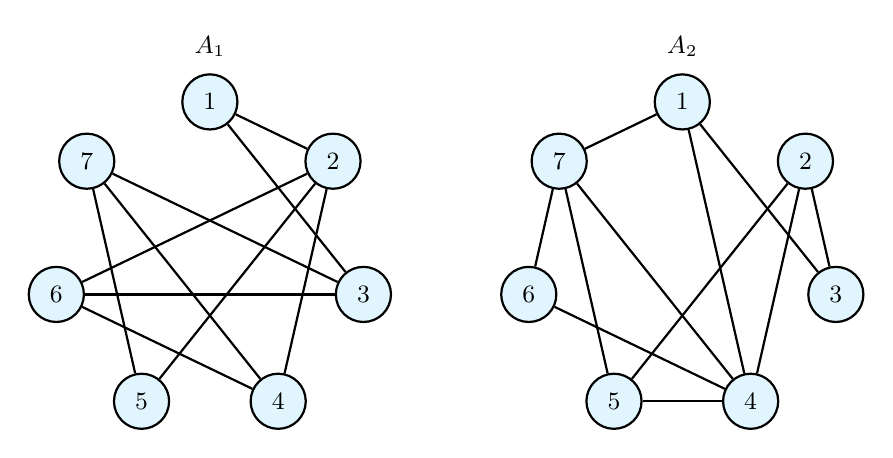
\begin{tikzpicture}[line width=0.8pt,font=\small]
\node[vertex] (v1) at (0.0,2.0) {$1$};
\node[vertex] (v2) at (1.5637,1.247) {$2$};
\node[vertex] (v3) at (1.9499,-0.445) {$3$};
\node[vertex] (v4) at (0.8678,-1.8019) {$4$};
\node[vertex] (v5) at (-0.8678,-1.8019) {$5$};
\node[vertex] (v6) at (-1.9499,-0.445) {$6$};
\node[vertex] (v7) at (-1.5637,1.247) {$7$};
\draw (v1) -- (v2);
\draw (v1) -- (v3);
\draw (v2) -- (v4);
\draw (v2) -- (v5);
\draw (v2) -- (v6);
\draw (v3) -- (v6);
\draw (v3) -- (v7);
\draw (v4) -- (v6);
\draw (v4) -- (v7);
\draw (v5) -- (v7);\node at (0,2.7) {$A_1$};\begin{scope}[xshift=6cm]\node[vertex] (v1) at (0.0,2.0) {$1$};
\node[vertex] (v2) at (1.5637,1.247) {$2$};
\node[vertex] (v3) at (1.9499,-0.445) {$3$};
\node[vertex] (v4) at (0.8678,-1.8019) {$4$};
\node[vertex] (v5) at (-0.8678,-1.8019) {$5$};
\node[vertex] (v6) at (-1.9499,-0.445) {$6$};
\node[vertex] (v7) at (-1.5637,1.247) {$7$};
\draw (v1) -- (v3);
\draw (v1) -- (v4);
\draw (v1) -- (v7);
\draw (v2) -- (v3);
\draw (v2) -- (v4);
\draw (v2) -- (v5);
\draw (v4) -- (v5);
\draw (v4) -- (v6);
\draw (v4) -- (v7);
\draw (v5) -- (v7);
\draw (v6) -- (v7);\node at (0,2.7) {$A_2$};\end{scope}
\end{tikzpicture}\end{document}
